% !TeX root = document.tex
% !TeX encoding = UTF-8 Unicode

\chapter{Theoretical Foundations}%
\label{chp:theoretical-foundations}

This work presents a Command Governor-based control strategy, based on the
concept of region of attraction, for switched systems. Thus, those are the main
concepts involved in this work and will be further explained in the following
sections.

\section{Switched Systems}%
\label{sec:switched-systems}

A switched system is a system composed of many subsystems, called modes, and a
mode-transition rule. It is often used to divide non-linear systems into many
linear systems around different operation points, creating linear
approximations, which are active one at a time. Differently from switching
systems, in which mode transition can happen arbitrarily, in the switched
system, a supervisor orchestrates
them~\parencite{lucia.franzè:stabilization,liberzon.morse:basic}.

A linear switched system can be described as follows
%
\begin{align}
  \dot{x}(t) & = A_{\sigma(t)}x(t) + B_{\sigma(t)}u(t), \\
  y(t)       & = C_{\sigma(t)}x(t) + D_{\sigma(t)}u(t),
\end{align}
%
where \(\sigma(t):t>0\rightarrow\mathbb{K}=\{1,\ldots,N\}\) is the switching function.
\(A_{i}, B_{i}, C_{i}\) and \(D_{i}\) are real matrices and represent
linearizations around different operation points. On the other hand, there are
also nonlinear switched systems with the form
%
\begin{align}
  \dot{x}(t) & = f_{\sigma(t)}(t,x(t),u(t)), \\
  y(t)       & = g_{\sigma(t)}(t,x(t)),
\end{align}
%
but those will not be discussed here. In both cases, \(t_{k}:k\in\mathbb{N}\) is
the switching instant.

There are two classes of switching functions: pertubation and control. For the
former, given \(J(\sigma)\) a switching criterion and
\(\mathcal{D}_{T}=\sigma(\cdot):t_{k+1}-t_{k}\ge{}T~\forall{}~k\in{}\mathbb{N}\), we solve
%
\begin{equation}
  \sigma = \sup_{\sigma\in\mathcal{D}_{T}} J(\sigma),
\end{equation}
%
and for the later, which is the one of interest for us, given \(\mathcal{S}\)
the set of all stabilizing switching functions, we solve
%
\begin{equation}
  \sigma = \inf_{\sigma\in\mathcal{S}} J(\sigma).
\end{equation}

This is, however, a very broad definition. In plain english, the pertubation
switching function finds the worse-case scenario (the admissible pertubation
depends on the magnitude of \(T\)) and the control the best-case. To define
stabilizing switching functions, let us analyse the stability of switched
systems.

The linear switched system is not guaranteed to be stable even if all subsystems
are stable~\parencite{liberzon.morse:basic}. This happens because the switching
signal itself is a source of instability, as the subsystems might behave
differently and diverge or start cycling under constant switching. This can also
be seen if you consider the set \(\{A_{1}, A_{2}, \ldots, A_{N}\}\) to be the
vertices of a polytope, as the system will be instantaneously jumping between
the vertices~\parencite{geromel.colaneri:stabilization}.

If we consider the system to be a polytope and can find \(P\succ{}0\) such that
%
\begin{equation}
  A_{i}^{\top}P+PA_{i} \prec{} 0,
\end{equation}
%
then the system is stable under arbitrary
switching~\parencite{geromel.deaecto:stability}. However, this is a conservative
solution and might yield very small regions of attraction. A more desirable
result is to have a mode dependent Lyapunov cadidate function leading to
%
\begin{equation}
  A_{i}^{\top}P_{i}+P_{i}A_{i} \prec{} 0,
\end{equation}
%
which is, however, only stable under arbitrary switching, from any mode \(i\) to
any mode \(j\), if
%
\begin{align}
  V(x(t_{k+1})) & = x^{\top}(t_{k+1})P_{j}x(t_{k+1})                                        \\
                & = x^{\top}(t_{k})e^{A^{\top}_{i}T_{k}}P_{j}xe^{A_{i}T_{k}}(t_{k})         \\
                & < x^{\top}(t_{k})e^{A^{\top}_{i}(T_{k}-T)}P_{i}xe^{A_{i}(T_{k}-T)}(t_{k}) \\
                & < x^{\top}(t_{k})P_{i}x(t_{k})                                            \\
                & = V(x(t_{k})),
\end{align}
%
implying that all subsystems must be
stable~\parencite{geromel.colaneri:stabilization}.

The solutions discussed so far allow arbitrary switching, but a large class of
systems will not satisfy the required condition. If the switching is assumed to
not be arbitrary, one can create a switching rule that will guarantee stability.
There is a class of such rules called slow-switching. The dwell-time is a rule
of this class requiring \(t_{k+1}-t_{k}>T\), that is, the system must remain on
a mode for \(T\) seconds before switching again. This time is counted from the
moment the reference changes. The goal is to minimize \(T\), minimizing the time
the system has to
wait~\parencite{chesi.colaneri.ea:computing,franzè.lucia.ea:command,liberzon.morse:basic}.
Note that there is one dwell-time \(T\) for each mode.

Other ways of guaranteeing switching stability exists.
See~\textcite{geromel.deaecto:stability,liberzon.morse:basic,geromel.colaneri:stabilization}.

\section{Command Governor}%
\label{sec:command-governor}

\subsection{System Description}%
\label{subsec:system-description}

A linear, switched, discrete-time system given in the state-space representation
can be described as follows
%
\begin{equation}
  \label{eq:state-space}
  \begin{aligned}
    x(k+1) & = A_{i}x(k)+B_{i}u(k), \\
    y(k)   & = C_{i}x(k)+D_{i}u(k), \\
    c(k)   & = E_{i}x(k)+F_{i}u(k),
  \end{aligned}
\end{equation}
%
where \(x(k)\in\mathbb{R}^n\) is the state vector, \(y(k)\in\mathbb{R}^p\) is the
output, \(c(k)\in\mathbb{R}^{n_c}\) is the constrained or weight output, the
matrices \(A_{i}\in\mathbb{R}^{n\times{}n}\), \(B_{i}\in\mathbb{R}^{n\times{}n_u}\),
\(C_{i}\in\mathbb{R}^{n_y\times{}n}\), and \(D_{i}\in\mathbb{R}^{n_y\times{}n_u}\) concern the
system's dynamic and output, matrices \(E_{i}\in\mathbb{R}^{n_c\times{}n}\) and
\(F_{i}\in\mathbb{R}^{n_c\times{}n_u}\) concern the constrained output and are chosen
by the designer to take into account the constraints associate with the state
and control signal. The sub-index \(i = 1,\ldots,N\) refers to the active model.

\subsection{Command Governor}%
\label{subsec:cg}

The Command Governor (\CG{}) is an add-on technique that extends existing
controllers with constraint enforcement. It uses the system model to predict
states given a reference \(r(k)\) and computes the virtual reference \(g(k)\)
closest to \(r(k)\) that keeps the system constrained.
Figure~\ref{fig:cg-schematic} presents a block diagram containing a single \CG{}
unit.

% !TeX root = ../document.tex
% !TeX encoding = UTF-8 Unicode

\begin{figure}[ht!]
  \centering
  \resizebox*{\linewidth}{!}{%
    \begin{tikzpicture}[node distance=1cm,block/.style={align=center,draw,shape=rectangle,very thick,minimum height=2em, minimum width=3em},>={Stealth}]

      \node (r)  []                      {\(r(k)\)};
      \node (cg) [block, right=of r]     {Command\\Governor};
      \node (C)  [block, right=of cg]    {Primal\\Controller};
      \node (G)  [block, right=of C]     {System};
      \node (y)  [right=of G.north east] {\(y(k)\)};
      \node (c)  [right=of G.south east] {\(c(k)\)};
      \node (e)  [below=of C]            {\(\begin{bmatrix}x_{c}(k)\\x(k)\end{bmatrix}\)};
      \node [draw=blue,rectangle,dashed,fit=(C) (G) (e)] {};

      \draw [->, thick] (r) -- (cg);
      \draw [->, thick] (cg) -- node [above] {\(g(k)\)} (C);
      \draw [->, thick] (C) -- node (u) [above] {\(u(k)\)} (G);

      \draw [->, thick] ([yshift=-3mm]G.north east) -- (y.west);
      \draw [->, thick] ([yshift=3mm]G.south east) -- (c.west);
      \draw [->, thick] (G) |- node (x) [near start, above right] {\(x(k)\)} ([yshift=1em]e.south east);
      \draw [->, thick] (x) -| ([xshift=5mm]C.south);
      \draw [->, thick] (C) -- node [left] {\(x_{c}(k)\)} (e.north);
      \draw [->, thick] (e.west) -| (cg.south);
    \end{tikzpicture}%
  }
  \caption[Command Governor Block Diagram.]{Command Governor Block Diagram. The
    system's and controller's states are fedback to constraint the output
    \(c(k)\).}%
  \label{fig:cg-schematic}
\end{figure}


The process diagram in Figure~\ref{fig:pi-controller-diagram} is simplified here
as the dashed blue square. The reference is not an input of the process, but of
the \CG{} and the output of the \CG{} is the input of the process. The \CG{}
block has two inputs: the reference and the augmented state vector, a
concatenation of the controller's state \(x_{c}(k)\) and the system's state
\(x(k)\).

An optmization procedure, described below, calculates the reference \(g(k)\)
which keeps the system output \(c(k)\) within a predefined region, called the
constraint. In the system defined in Equation~\eqref{eq:state-space} the
constraint is applied to a linear combination of the states and inputs of the
system. \(c(k)\) is not fed back to the \CG{} because the information needed to
calculate it is already used during the design of the \CG{} logic, so it can be
reconstructed from the augmented vector.

In what follows we use the sets \(\mathcal{C}\), \(\mathcal{W}\), and
\(\mathcal{V}(x(k))\) defined as follows:

\begin{enumerate}
  \item \(\mathcal{C}\) is the set of restrictions, which contains all allowed
        values of \(c(k)\).
  \item \(\mathcal{W}\) is the set of all constant references \(\omega{}\) that keep
        \(c(k)\) constrained on the steady-state.
        \[\mathcal{W} = \{\omega\in\mathbb{R}^{n_y}:
          c(k)\in\mathcal{C},k\rightarrow\infty{}\}.\]
  \item \(\mathcal{V}(x(k))\) is the set of \(\omega{}\) values which ensures that
        the constrained output belongs to \(\mathcal{C}\) during the transitory
        \[
          \mathcal{V}(x(k))=\{\omega\in\mathcal{W}:c(k)\in\mathcal{C},0<k\leq{}k_0\},
        \]
\end{enumerate}

We write the set \(\mathcal{V}(x(k))\) in terms of convex constraints on the virtual
reference, the \(k_{0}\) future states, the minimization of the distance to the
desired reference, and actuator saturation bound.

The output of the Command Governor is given by the following convex optimization
procedure:

\begin{equation}
  \begin{aligned}
    g(k)=\argmin_{\omega\in\mathcal{V}(x(k))} & \norm{\omega-r(k)}^2_\Psi
  \end{aligned}
  \label{eq:cg}
\end{equation}
%
where \(\Psi{}\) is a semi-definite positive weighing matrix and \(g(k)\) is the
virtual reference closest to the desired reference, not allowing the system to
violate the constraints. Observe that the set \(\mathcal{V}(x(k))\) is defined by
evolving the system in closed-loop, without disturbances, a number \(k_0\) of
samples ahead, and testing if the state sequence do not violate constraints.

\subsection{Supervisor}%
\label{subsec:supervisor}

The supervisor is responsible for selecting which \(i\)-th \CG{} is currently
active. Figure~\ref{fig:supervisor-schematic} shows its block diagram, in which
we see that all \CG{}s are continuously updated, but only \(\CG{}_{3}\) is
active, sending control signals to the system. The policy for switching \CG{}s
is problem-dependent. It might be another controller giving better performance,
according to some metric, or being able to access a state-space region. Note
that each \CG{} unit has its \(\mathcal{C}_{i}\), \(\mathcal{W}_{i}\) and
\(\mathcal{V}(x(k))_{i}\) sets.

\begin{figure}[ht!]
  \centering
  \captionsetup{justification=centering}
  \begin{tikzpicture}[auto,node distance=1cm,>={Stealth},block/.style={draw,rectangle,minimum height=2em,minimum width=4em,thick},sum/.style={draw,circle,thick},point/.style={coordinate},dot/.style={draw,thick,circle,minimum size=0.5em},tight/.style={inner sep=0pt,outer sep=0pt}]
    \node (cg2) [block]              {\(CG_{2}\)};
    \node (C2)  [block,right=of cg2] {\(PC_{2}\)};
    \node (X2)  [tight,below=of C2]  {\(\begin{bmatrix}x_{C2}(k)\\x(k)\end{bmatrix}\)};
    \node [draw,rectangle,dashed,fit=(cg2) (C2) (X2)] {};
    \draw [->,thick] (cg2) -> node [below] {\(g_{2}(k)\)} (C2);
    \draw [->,thick] (C2) -> node [swap] {\(x_{C2}(k)\)} (X2);
    \draw [->,thick] (X2) -| (cg2);

    \node (cg3) [block,above=3cm of cg2] {\(CG_{3}\)};
    \node (C3)  [block,right=of cg3]     {\(PC_{3}\)};
    \node (X3)  [tight,below=of C3]      {\(\begin{bmatrix}x_{C3}(k)\\x(k)\end{bmatrix}\)};
    \node [draw,rectangle,dashed,fit=(cg3) (C3) (X3)] {};
    \draw [->,thick] (cg3) -> node [below] {\(g_{3}(k)\)} (C3);
    \draw [->,thick] (C3) -> node [swap] {\(x_{C3}(k)\)} (X3);
    \draw [->,thick] (X3) -| (cg3);

    \node (cg1) [block,below=3cm of cg2] {\(CG_{1}\)};
    \node (C1)  [block,right=of cg1]     {\(PC_{1}\)};
    \node (X1)  [tight,below=of C1]      {\(\begin{bmatrix}x_{C1}(k)\\x(k)\end{bmatrix}\)};
    \node [draw,rectangle,dashed,fit=(cg1) (C1) (X1)] {};
    \draw [->,thick] (cg1) -> node [below] {\(g_{1}(k)\)} (C1);
    \draw [->,thick] (C1) -> node [swap] {\(x_{C1}(k)\)} (X1);
    \draw [->,thick] (X1) -| (cg1);

    \node (supervisor) [block,above left=of cg3,draw=orange] {Supervisor};
    \node (r) [left=of supervisor] {\(r(k)\)};
    \draw [->,thick] (supervisor) |- node [near start, above left] {\(r'(k)\)} (cg1);
    \draw [->,thick] (supervisor) |- (cg2);
    \draw [->,thick] (supervisor) |- (cg3);

    \node (sw1) [tight,dot,right=2cm of C2]          {};
    \node (sw2) [tight,dot,above right=0.5em of sw1] {};
    \node (sw3) [tight,dot,below right=0.5em of sw1] {};
    \node (sw4) [point,right=1em of sw1]             {};
    \node (sw5) [point,right=1em of sw4]             {};
    \node (switch) [draw,rectangle,tight,fit=(sw1) (sw2) (sw3) (sw5),thick] {};
    \draw [thick] (sw5) -- (sw4) -- (sw2);

    \node (system) [block,right=1.5cm of switch] {System};
    \node (y) [right=of system] {\(y(k)\)};

    \draw [->,thick] (r) |- (supervisor);
    \draw [->,thick,dotted,draw=orange] ([yshift=0.75em]supervisor.south east) -| ([xshift=-0.5em]switch.north east);
    \draw [->,thick] (system) -- (y);
    \draw [->,thick,draw=blue] (switch) -- node {\(u_{i}(k)\)} (system);
    \draw [->,thick,draw=blue] (C3.east) -| node [below left] {\(u_{3}(k)\)} (sw2.north);
    \draw [->,thick,draw=blue] (C2.east) --  node {\(u_{2}(k)\)} (sw1.west);
    \draw [->,thick,draw=blue] (C1.east) -| node [above left] {\(u_{1}(k)\)} (sw3.south);
    \draw [->,thick,draw=red] (system) |- ([yshift=0.75em]X1.south east);
    \draw [->,thick,draw=red] (system) |- node [above left] {\(x(k)\)} ([yshift=0.75em]X2.south east);
    \draw [->,thick,draw=red] (system) |- node [above left] {\(x(k)\)} ([yshift=0.75em]X3.south east);
    \draw [->,thick,draw=red] (system) |- ([yshift=-0.75em]supervisor.north east);
    \draw [->,thick,draw=red] (system) |- ++(-1cm,-5cm) -| ([xshift=-1em]C1.south east);
    \draw [->,thick,draw=red] (system) |- ++(-1cm,-1cm) -| ([xshift=-1em]C2.south east);
    \draw [->,thick,draw=red] (system) |- ++(-1cm,3cm)  -| ([xshift=-1em]C3.south east);
  \end{tikzpicture}%
  \caption{Supervisor Block Diagram.}%
  \label{fig:supervisor-schematic}
\end{figure}


However, even if the policy allows the change, it will not be admissible if
\(x(k)\not\in\mathcal{X}_i\cap{}\mathcal{X}_j\), where
%
\begin{equation}
  \mathcal{X}_i =
  \left\{
  x\in\mathbb{R}^n | \begin{bmatrix}\omega\\x\end{bmatrix} \in
  \mathcal{Z}_i \textrm{ for at least one } \omega\in\mathbb{R}^{n_y}
  \right\}
\end{equation}
%
is the set of all states that can be steered to an equilibrium point without
constraint violation, with
%
\begin{equation}
  \mathcal{Z}_i =
  \left\{
  \begin{bmatrix}r\\x\end{bmatrix}
  \in\mathbb{R}^{n_y+n} | c(k)\in\mathcal{C}_i,
  \forall{}k\in\mathbb{Z}^+
  \right\}
\end{equation}
%
being the admissible output set.

A switched system must have many \CG{} units, each of them with its constraint
region. A generic \CG{} switch from \(\CG{}_{i}\) to \(\CG{}_{j}\), denoted
\(\CG{}_i\rightarrow{}\CG{}_j\), is admissible (with respect to the plant constraints) if
the two \CG{}'s domains have a nonempty intersection. If one wants to go from
\(\CG{}_1\) to \(\CG{}_3\) and there is no intersection, one must find a path
through other \CG{}s with nonempty intersections. Therefore the union of all
\CG{}'s domains cannot be a disconnected domain.

To change the active \CG{}, one needs to go to a point interior to the \CG{}'
domains intersection, called way-point. Such a point can be chosen arbitrarily
inside the intersection of regions defined by the constraints of the concerned
\CG{}s. However, it is better to use points in the central area, not so close to
the borders, to avoid problems involving disturbances and controller
sensitivity~\parencite{keel.bhattacharyya:robust}. All the paths from one \CG{}
to another can be calculated offline, for example, using graph
theory\parencite{ahuja.mehlhorn.ea:faster,pettie:new}. Such an aspect is now
handled in this work and, then, the path is assumed to be known.

In~\parencite{franzè.lucia.ea:command,lucia.franzè:stabilization} it has been
shown that any \(\CG{}\) switch, e.g. \(\CG{}_i\rightarrow{}\CG{}_j\) can be safely
accomplished (not violating the constraints) from any point belonging to the
intersection between the two \CG{}s' domains. Therefore, a possible way to
achieve a safe switch is to define a waypoint reference in the intersection set.
Once the plant trajectory, under the action of \(\CG{}_i\) is confined in the
intersection region, then \(\CG{}_j\) is activated.

This approach is a way of guaranteeing stability, as the dwell-time is
calculated to allow the switching to occur neither too soon nor too often,
giving enough time to the current controller to stabilize the system before
switching again. It is, however, a very conservative approach that assumes a
worst-case scenario. Although it might be necessary to stabilize some systems,
it is not always needed and may lead the convergence time to take longer.

\section{Region of Attraction}%
\label{sec:region-of-attraction}

The Region of Attraction is a definition which initiated with the work of the
French mathematician Henri Poincaré. He studied real, nonlinear differential
equations' behaviour, finding that the states' evolution in time is stable,
unstable or cyclic. However, he did not find proof, which was later given by the
Swedish mathematician Ivar Bendixson~\parencite{bendixson:sur}.

Differential equations which describe real-world dynamics needs to satisfy a
condition, which imposes a bound to its first derivative. In other words, the
rate of change of the differential equation must be limited. This is a special
form of function continuity called Lipschitz continuity. All differential
equations that represent the dynamics of a real-world, physical system satisfy
this condition. The condition is
%
\begin{equation}
  \label{eq:lipschitz}
  \norm{\frac{\partial{}f(x,t)}{\partial{}x}} \le L,
\end{equation}
%
where \(L\) is a real, positive constant, the rate of change. This condition is
important as it guarantees that the differential equation \(\dot{x}=f(x,t)\)
with initial condition \(x(t_{0})=x_{0}\) has a unique solution for every \(\delta\)
in \([t_{0}, t_{0}+\delta]\)~\parencite{donchev.farkhi:stability}. In other words,
the differential equation has only unique solutions.

For equations satisfying this condition, \textcite{bendixson:sur} presents the
definition of a region with interesting properties. First, he defines the
existence of a critical point for differential functions, which are points such
that the differential function's derivative are zero and remain zero as the time
goes to infinity. He then shows that there are two types of critical points:
stable and unstable. A stable critical point is such that all states on a given
neighbourhood converge to the point as time goes to infinity. For an unstable
critical point, they diverge. He then proceeds to show the existence of
limit-cycles, which are not critical points, but, for a differential equation
\(f(t,x,y)\), \(f(t,x,y)=f(t-t_{0},x,y)\), meaning that variables \((x,y)\), the
state, are repeating thenselves cyclic every \(t-t_{0}\) time units. Cycles can
be classified as stable or unstable by taking any of its points and applying the
same analysis as for critical points, with the addition that it may be
semi-stable, meaning that points inside the region convert and outside diverge,
or vice-versa.

To verify the type of a critical point, one can take the derivative of the
function and apply at the point. For a continuous-time differential equation,
the resulting values need to be negative for the point to be a stable critical
point, otherwise it is an unstable critical point. For a discrete-time system,
their absolute values must be smaller than one for the point to be stable.
Limit-cycles are only possible around critical points, so to test for their
existence on a function \(f(x)\), one must analyze the stability of the
critical-point and then define a region \(H(x)\), which contains the critical
point, and calculate the gradient (\(\nabla\)) of \(H(x)\) on \(f(x)\). The following
list sumarizes the possible outcomes:

\begin{enumerate}
  \item if the point is \textbf{unstable} and \(\nabla{}H(x)f(x) < 0\), then there is
        a \textbf{stable cycle} inside the region \(H(x)\);
  \item if the point is \textbf{unstable} and \(\nabla{}H(x)f(x) > 0\), then there is
        an \textbf{unstable cycle} inside the region \(H(x)\) \textbf{or no
          cycles};
  \item if the point is \textbf{stable} and \(\nabla{}H(x)f(x) < 0\), then there is a
        \textbf{semi-stable cycle} inside the region \(H(x)\) or \textbf{no
          cycles};
  \item if the point is \textbf{stable} and \(\nabla{}H(x)f(x) > 0\), then there is a
        \textbf{semi-stable cycle} inside the region \(H(x)\).
\end{enumerate}

Figure~\ref{fig:poincare-cycles} shows some possible gradients.
In~\ref{fig:semi-stable-cycle} there is a stable point and a semi-stable cycle.
Notice how all points inside the cycle converge to the origin (center of the
figure) and all points outside diverges. The cycle exists but is not stable, as
the state might either converge or diverge after some time.
In~\ref{fig:stable-cycle} the gradients are the opposite of the previous case,
resulting on a sustained cycle. Every initial state will converge to the cycle
and the state will keep looping forever. In~\ref{fig:stable-point} there is no
cycle, but there could be one. This is the most common case, specially when
working with linearizations. All states converge to the origin, regardless of
the initial state. Note that we do not know what happens outside the plotted
region. There could be a cycle hidden there, or the gradient might change
completely, so we cannot make any affirmation about the system's behaviour
outside the plotted region. You could call this region \(H(x)\) and it would be
a Region of Attraction.

\begin{figure}[!htb]
  \centering
  %
  \begin{subfigure}[b]{0.45\linewidth}
    \centering
    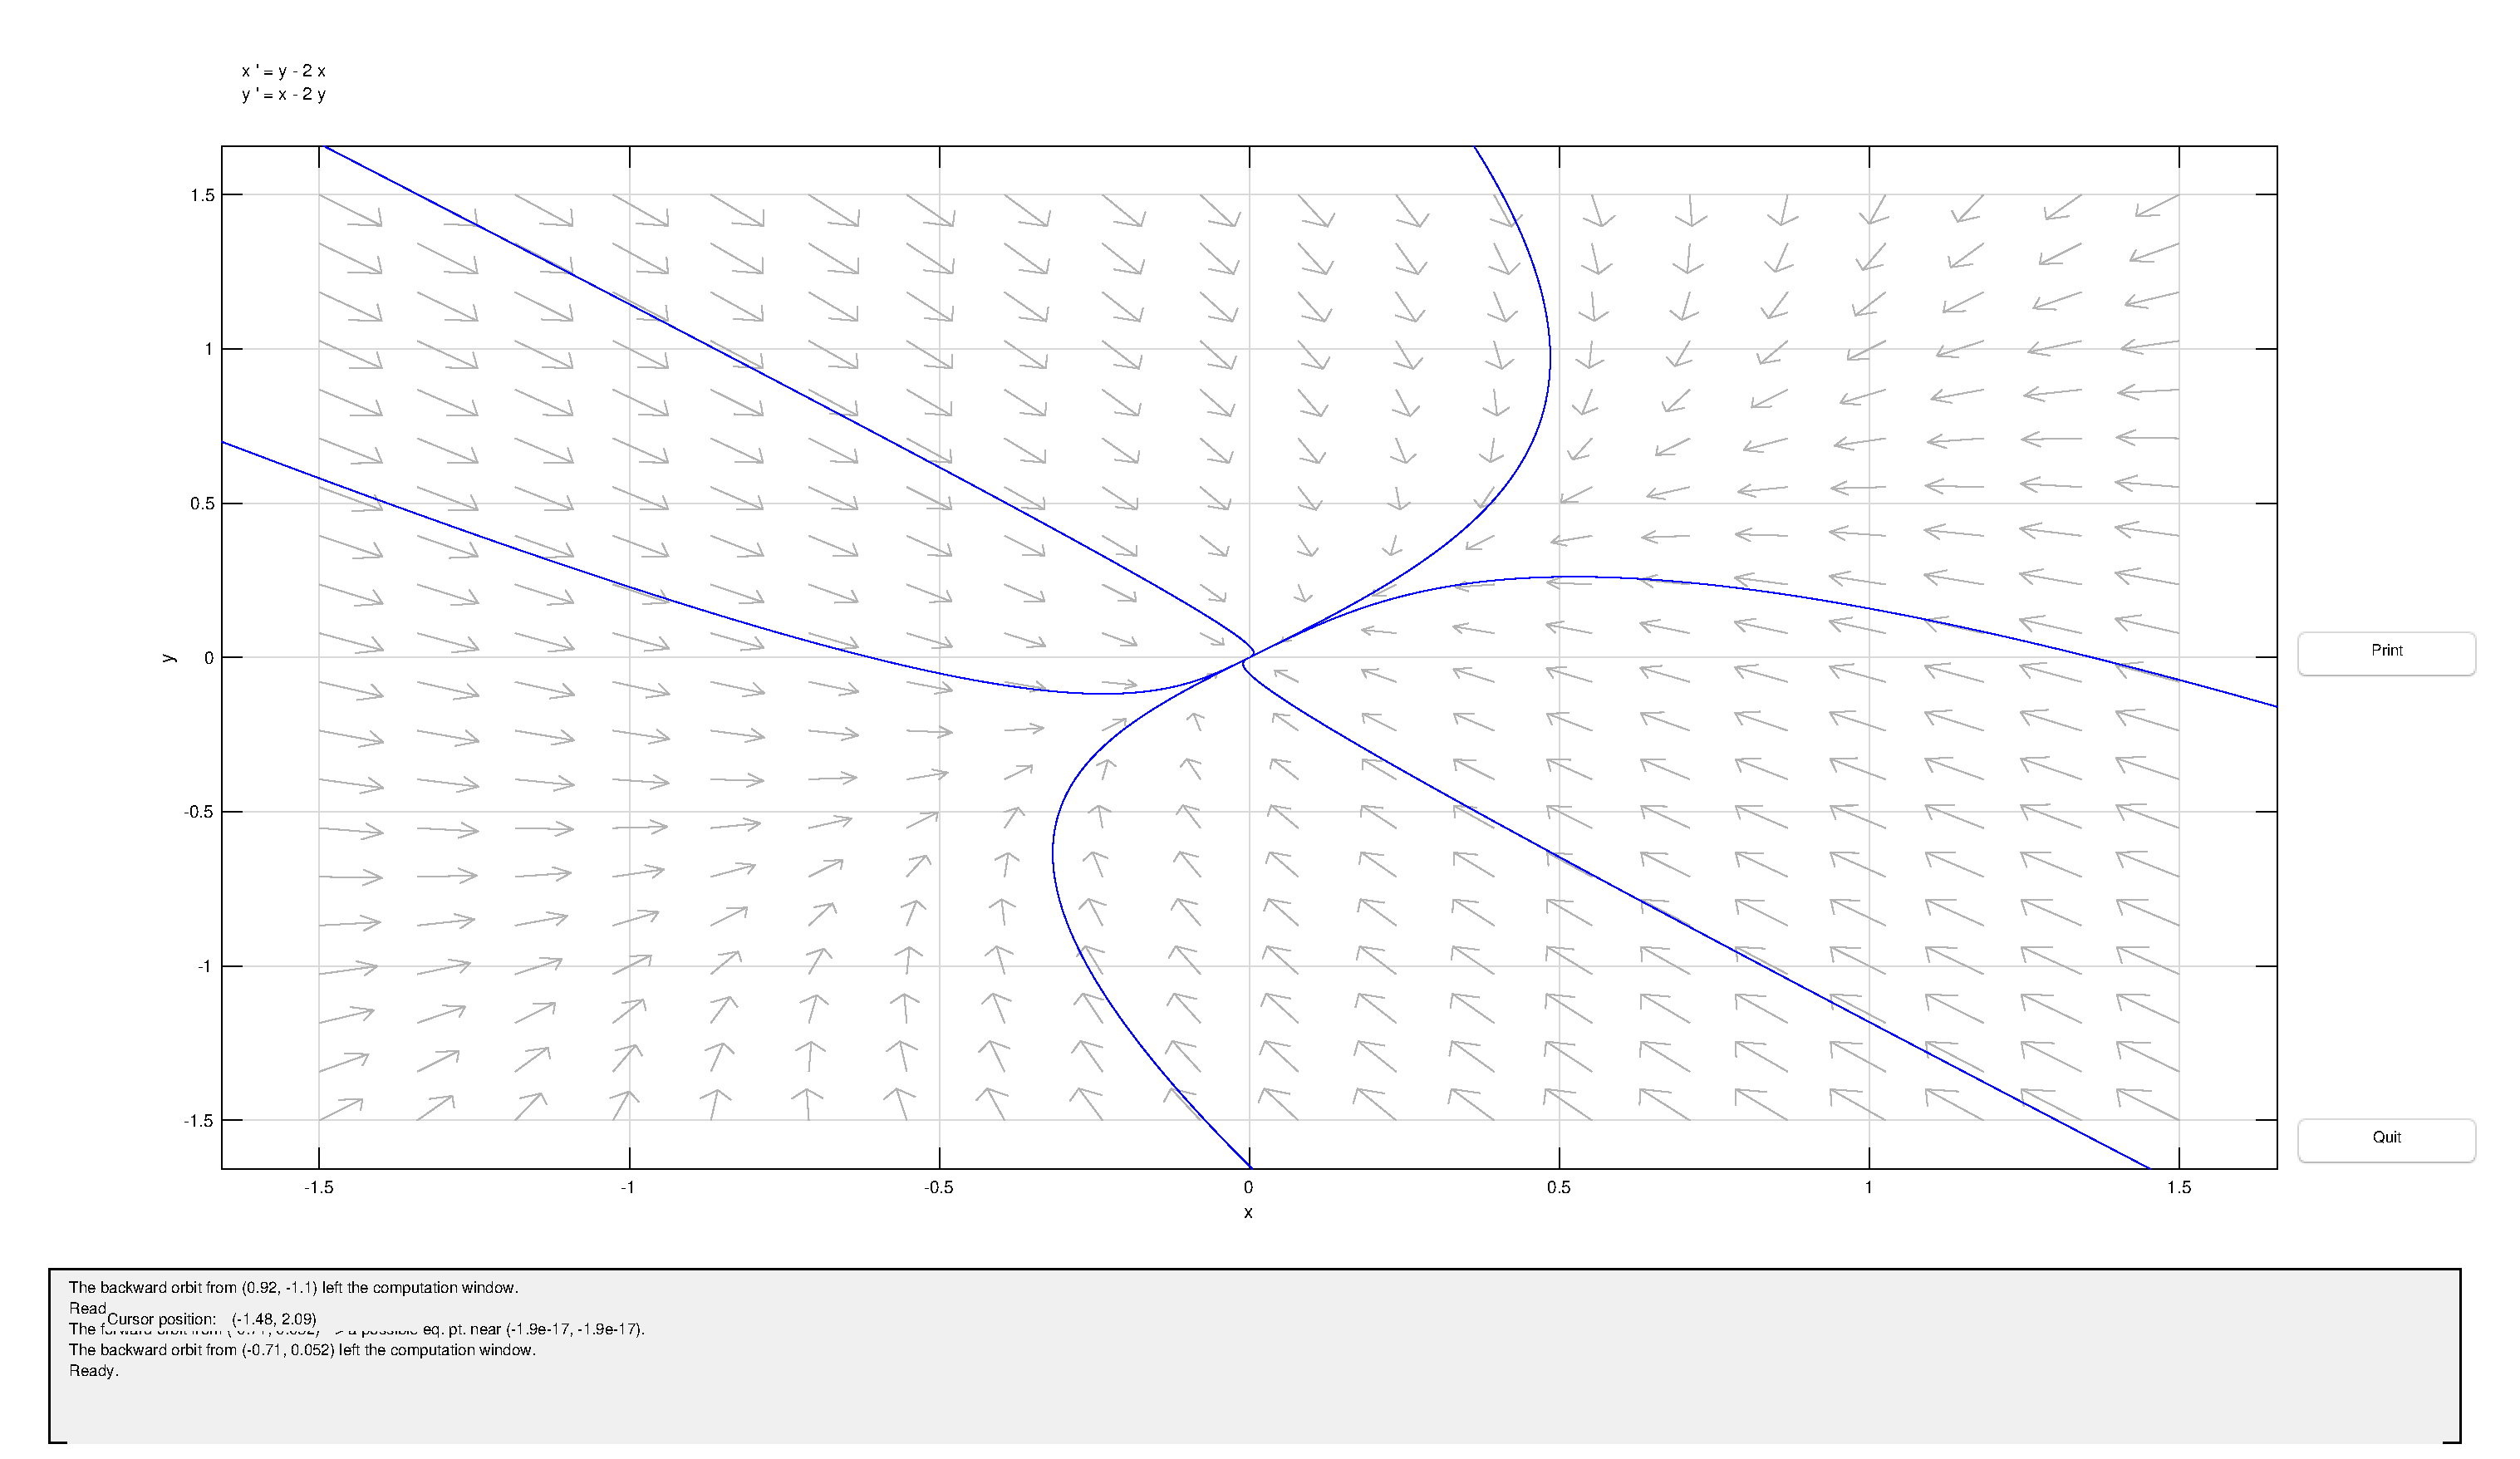
\includegraphics[trim=116 155 125 55,clip,width=\linewidth]{imgs/stable-point}
    \caption{Stable point}%
    \label{fig:stable-point}
  \end{subfigure}
  %
  \begin{subfigure}[b]{0.45\linewidth}
    \centering
    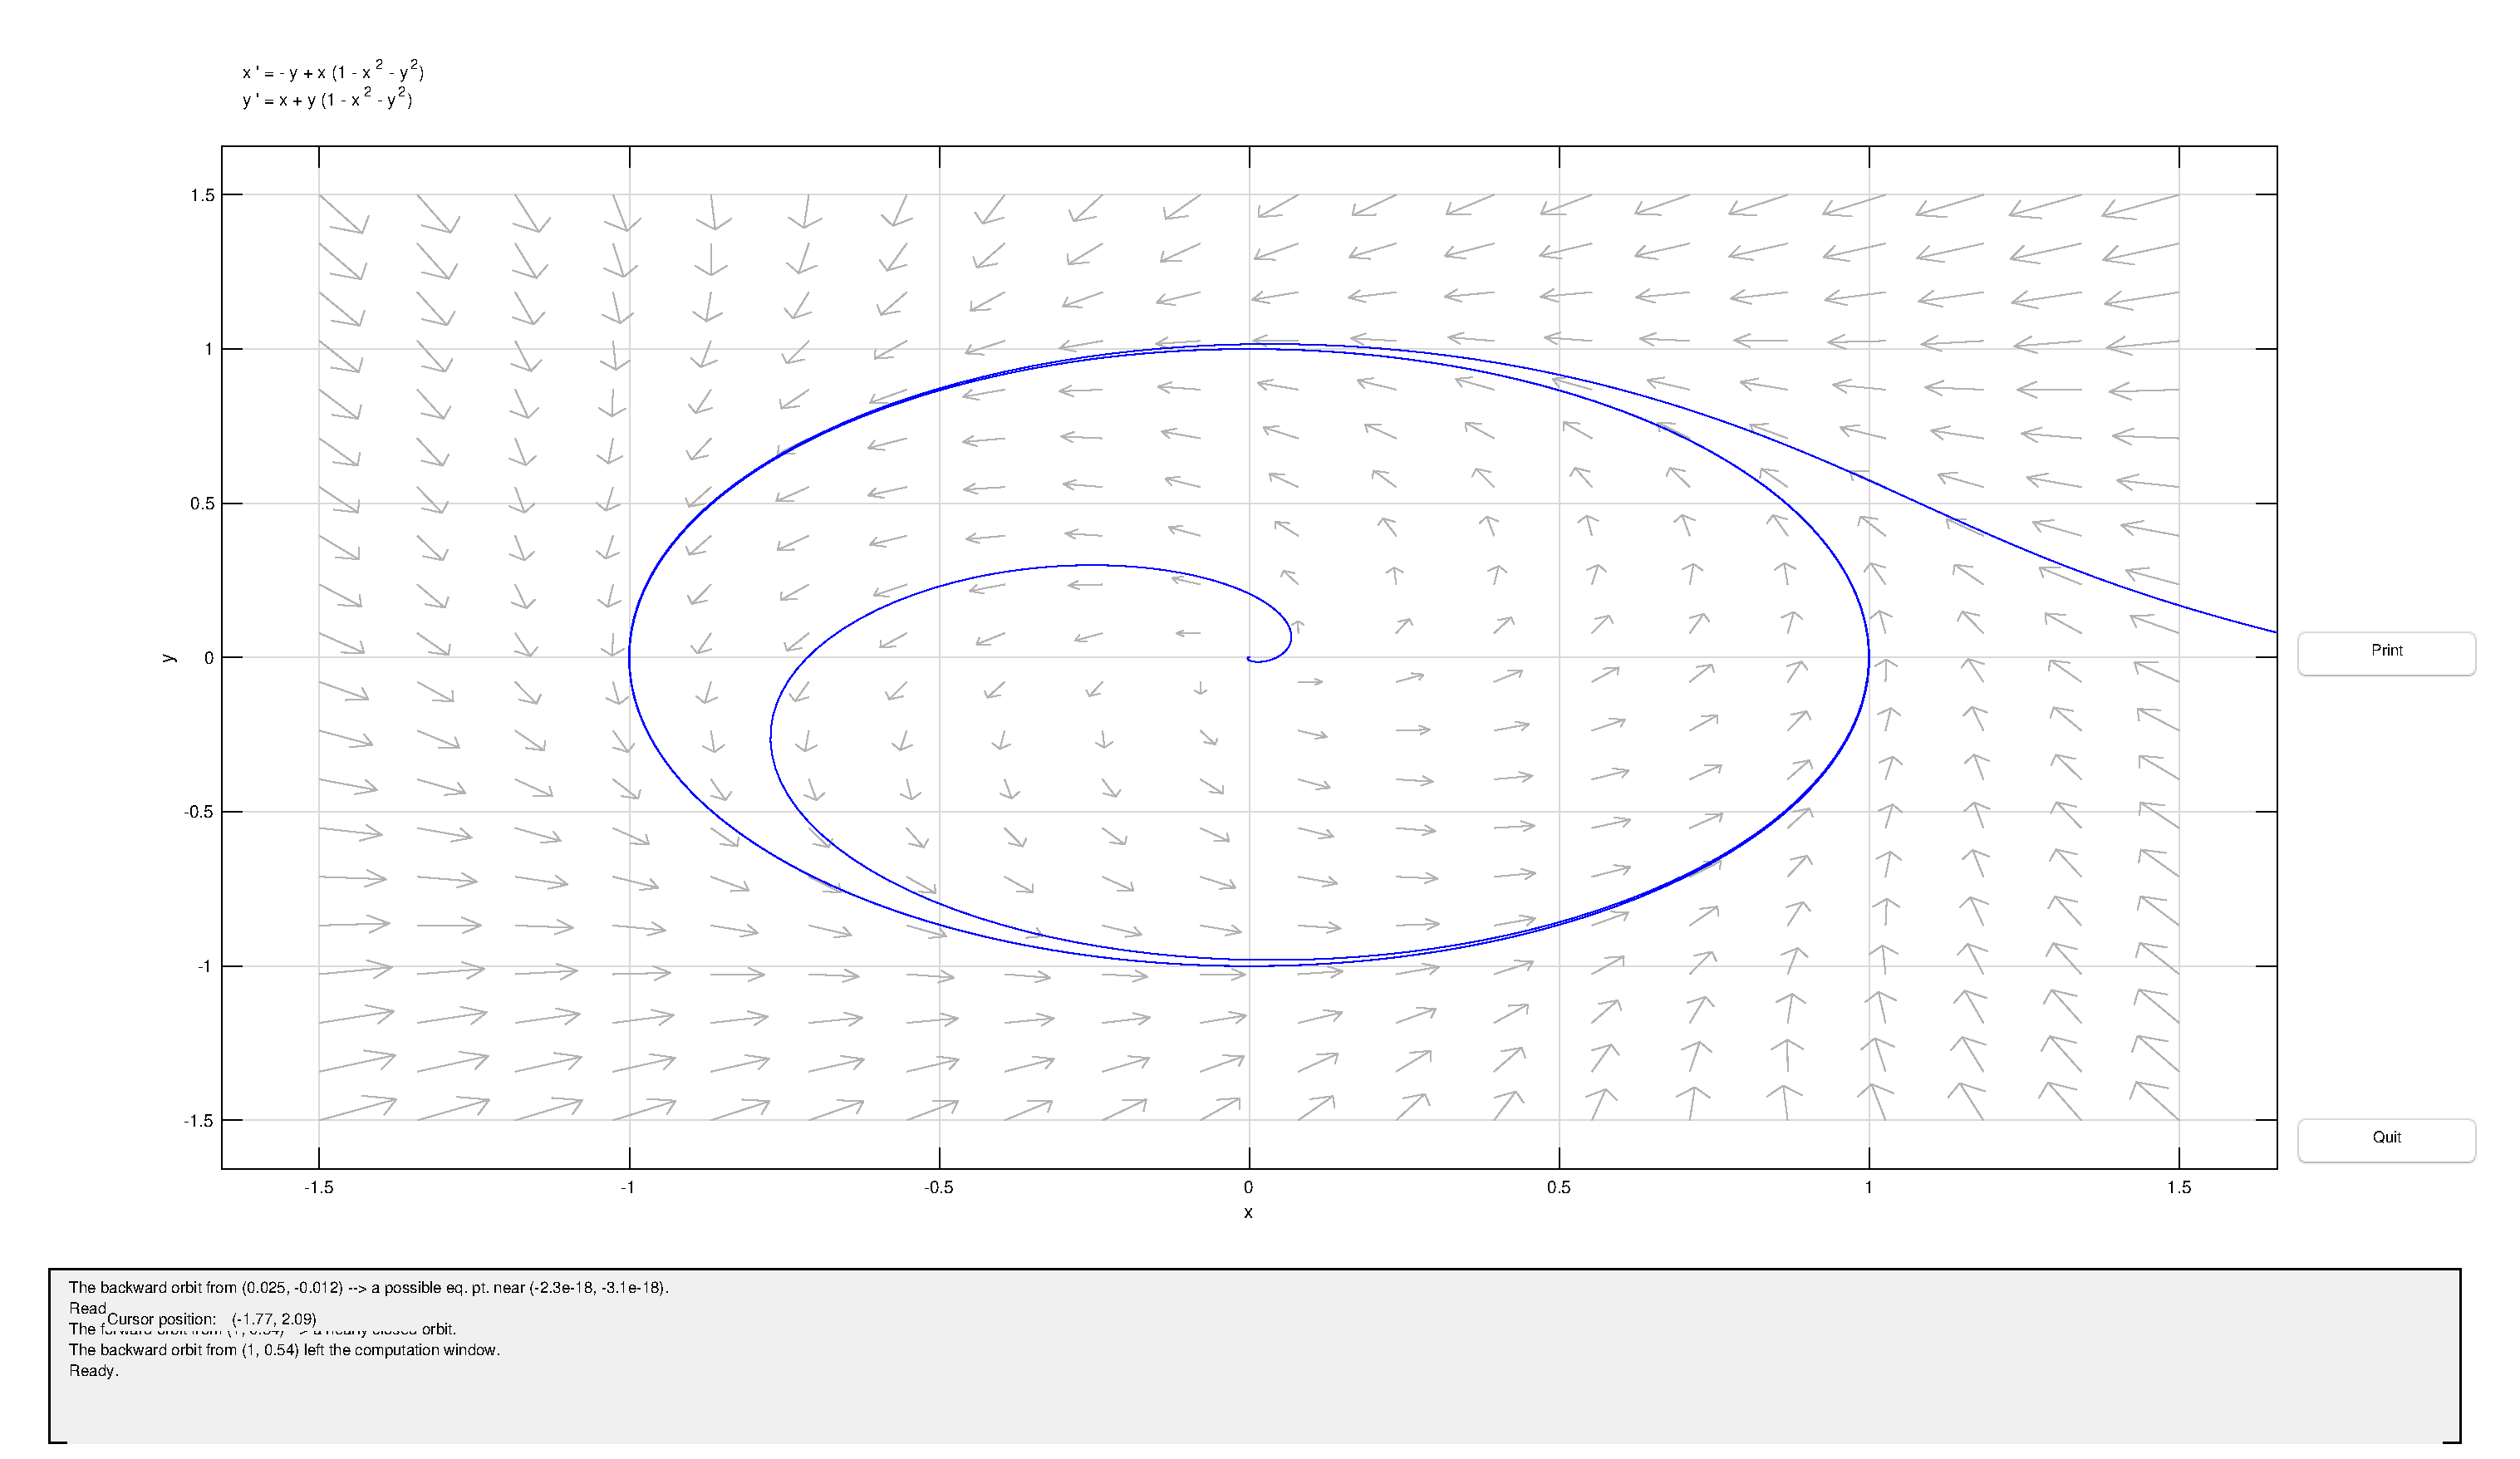
\includegraphics[trim=116 155 125 55,clip,width=\linewidth]{imgs/stable-cycle}
    \caption{Stable cycle}%
    \label{fig:stable-cycle}
  \end{subfigure}
  %
  \begin{subfigure}[b]{0.5\linewidth}
    \centering
    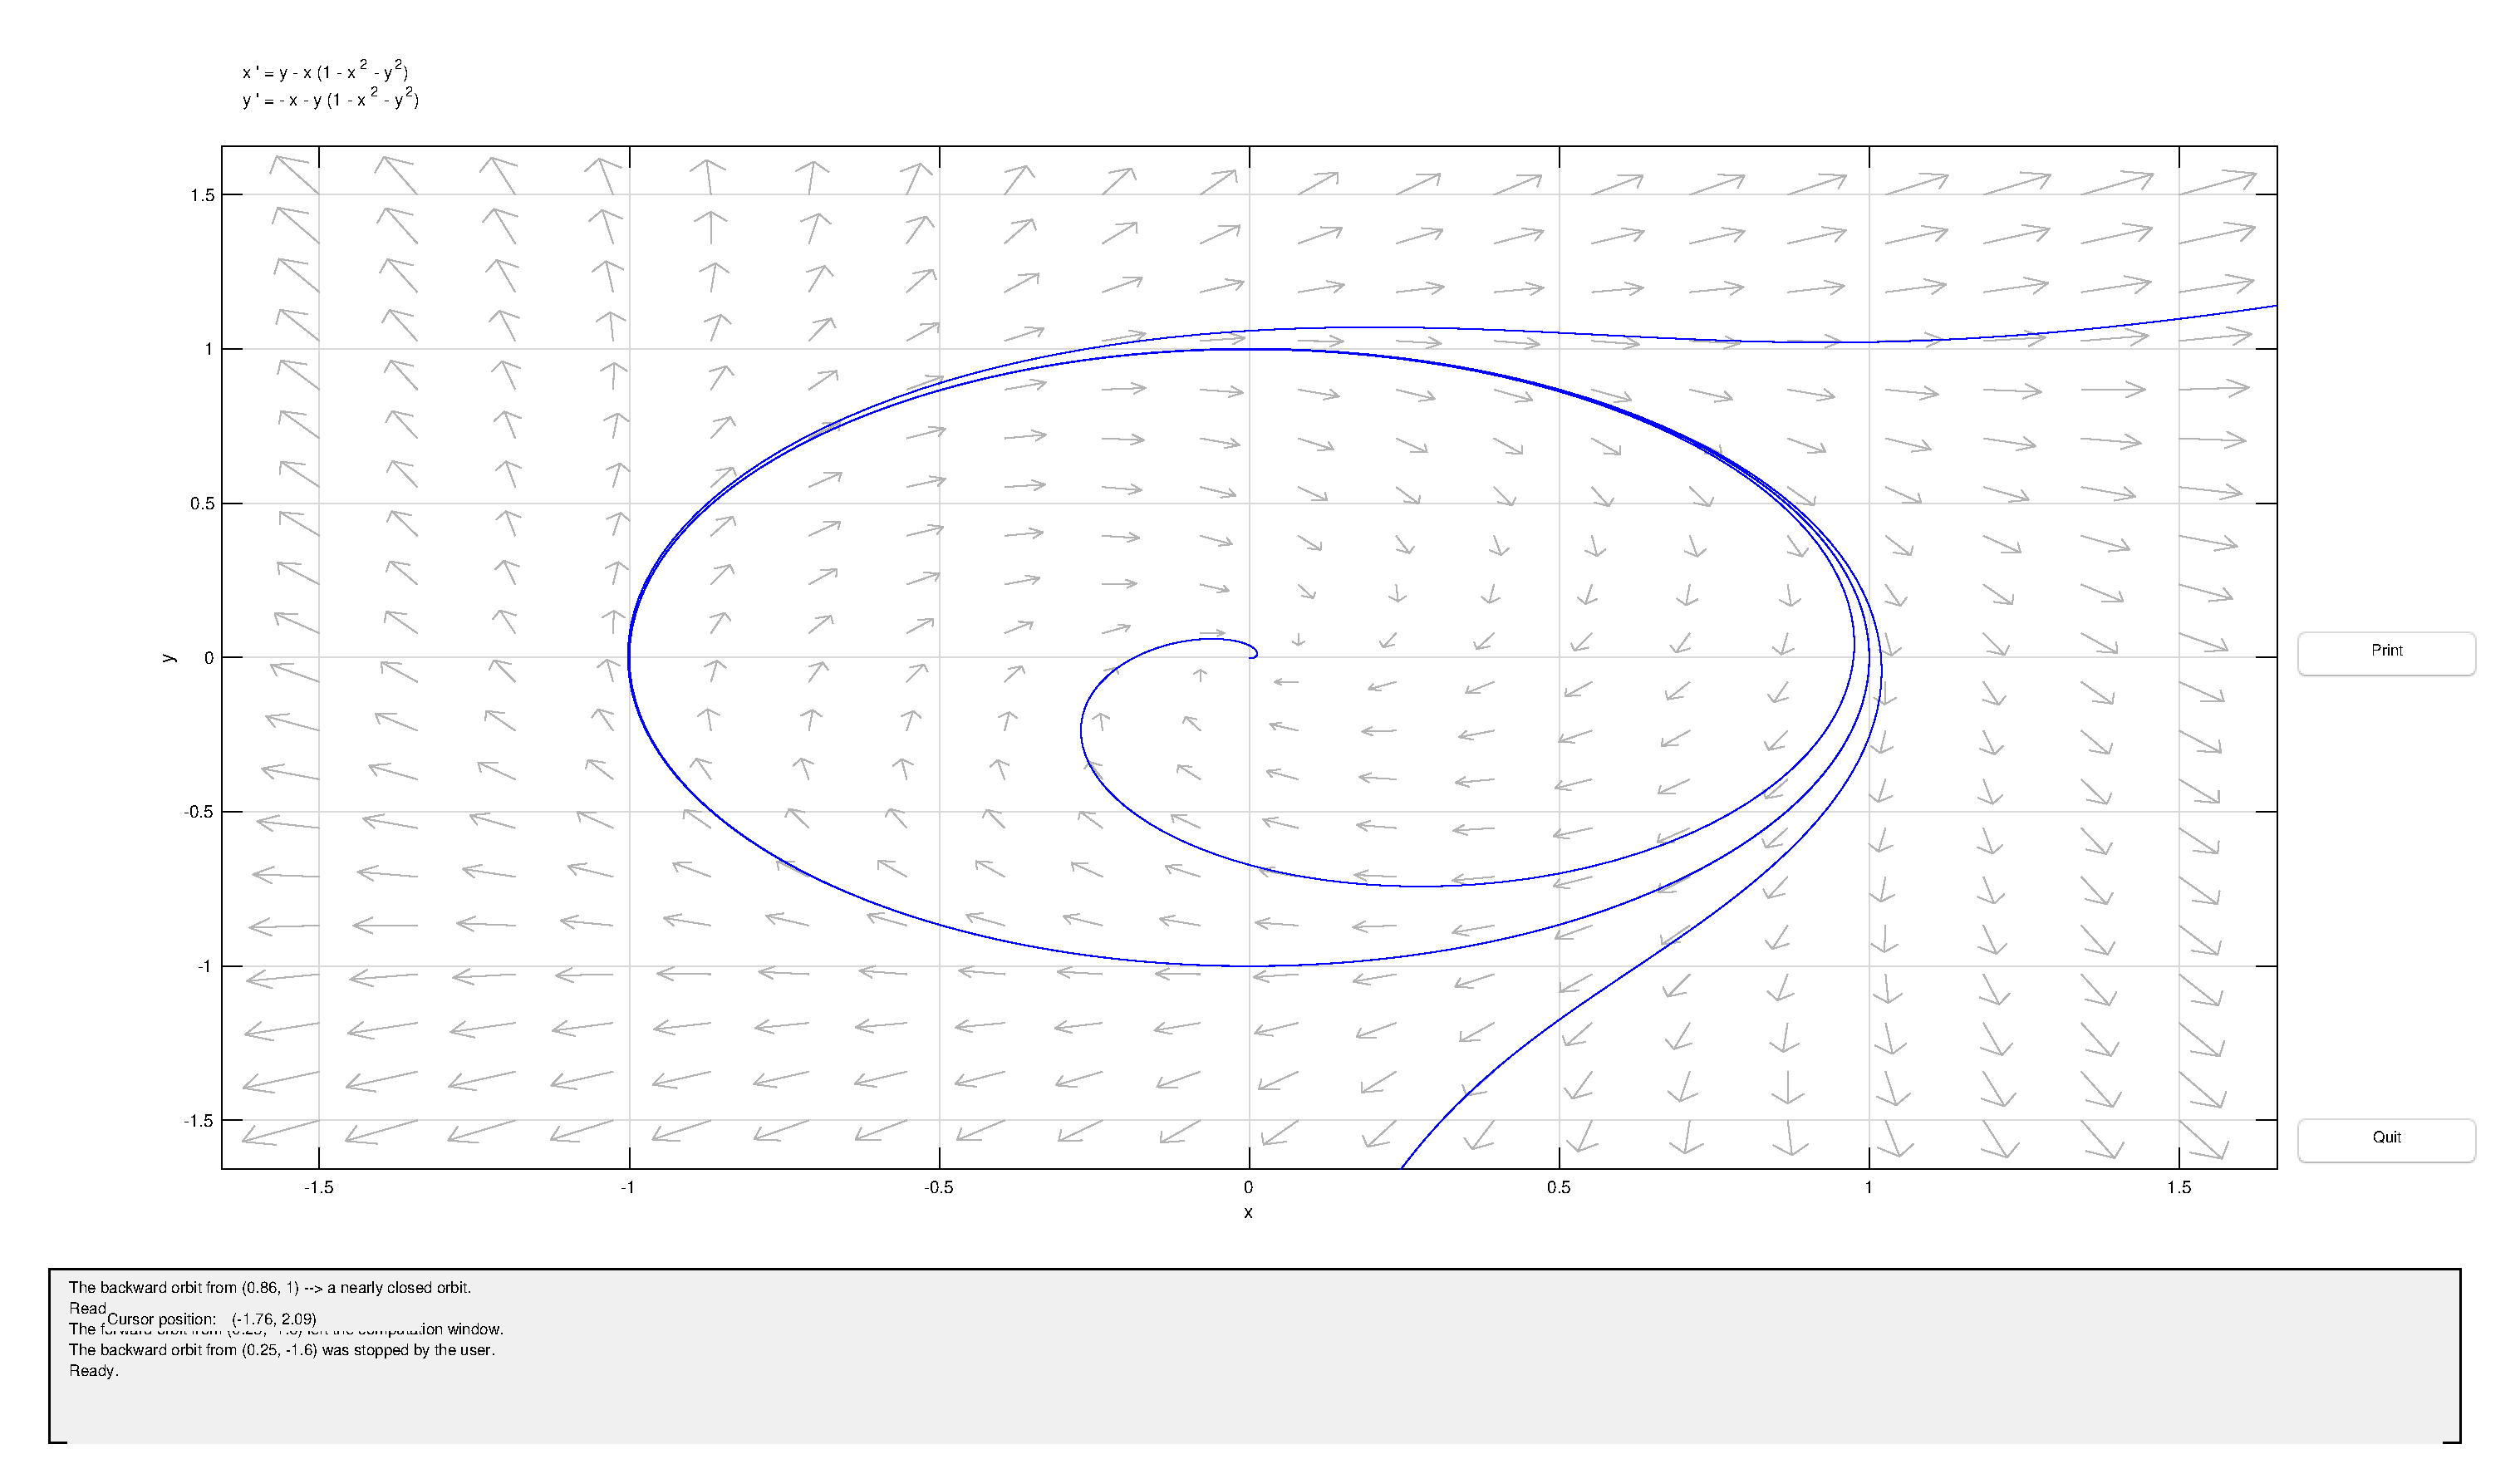
\includegraphics[trim=116 155 125 55,clip,width=\linewidth]{imgs/semi-stable-cycle}
    \caption{Semi-stable cycle}%
    \label{fig:semi-stable-cycle}
  \end{subfigure}
  %
  \caption[Different cycles' gradient maps.]{Different cycles' gradient maps.
    In~\ref{fig:stable-point} there is a stable critical point and all values
    converge to it. In~\ref{fig:stable-cycle} there is an unstable critical
    point and stable limit-cycle, so all values converge to the limit-cycle and
    remain cycling on its border. The vector field
    in~\ref{fig:semi-stable-cycle} is the contrary of that on the previous
    subfigure, and the values will only stay on the limit-cycle if they start
    there and there is no pertubation or noise, otherwise they will either
    converge to the critical point or diverge.}%
  \label{fig:poincare-cycles}
\end{figure}

\begin{definition}
  A Region of Attraction is the neighbourhood of a critical point which is
  forward invariant under the flow generated by it~\parencite[178]{milnor:on}.
\end{definition}

This definition allows limit-cycles to be inside the region of attraction, which
is undesirable for control purposes, where we expect the system to converge,
leading to a more restricted defition. Lyapunov's stability criteria states that
for the system \(\dot{x} = f(t, x)\), if there is a function \(V(x)\) such that
%
\begin{align}
  V(x)       & = 0 \iff x = 0,                                       \\
  V(x)       & > 0 \iff x \ne 0,                                     \\
  V(x_{1})   & >V(x_{2}) \iff x_{1} > x_{2}                          \\
  \dot{V}(x) & = \nabla{}V(x)f(x) \le 0 \phantom{0} \forall x \ne 0,
\end{align}
%
then the system is stable~\parencite{chen:linear,hespanha:linear}. Futhermore,
if \(\dot{V}(x)<0\), the system is asymptotically stable. In this context,
\(V(x)\) is an energy function, but its derivative reminds us of Poincaré's
theorem. In fact, Lyapunov's function can be seen as a more restricted form or
Poincaré's region, which always contains stable points or stable cycles inside
it. If the derivative is strictly negative, the region \(V(x)\) is guarantee to
not contain cycles~\parencite{chen:linear}. Because of this link between the two
theorems, Lyapunov's stability criteria is often used to estimate the region of
attraction.

In case of a linear system described by \(\dot{x} = Ax\), it is necessary and
sufficient to search for a function \(V(x)=x^{\top}Px\). It is the most used
candidate since it is easy to verify its positiviness: \(V(x)\ge{}0~\forall{}x\) if
\(P\) is SDP (semidefinte positive)~\parencite{bochnak.coste.ea:real}. It is
also a simple region to describe and derive, making it easy to use with LMI
tools. Note, however, that there are infinite possible regions, and
\(V(x)=x^{\top}Px\) is most certainly \textit{not} the largest region, making it a
conservative solution.
